\chapter{弱い相互作用、ビリアル補正、非完全微分}

\lectureoverview{まず測定と温度の操作的意味から始め、次に短距離相互作用が弱く加わったとき、希薄気体が理想気体の法則からどのようにずれるかを問う。分配関数はエネルギーと圧力への最初の相互作用補正を与え、その有効範囲を明らかにする。最後の数学的な補足では、完全微分、閉じたループ、および具体的な理想気体のテストを用いて、状態関数と経路に依存する熱および仕事を区別する。}

\section{計器が実際に測定するもの}

実験室の装置が直接自然の中に立ち入って抽象的な数学的変数を報告することはない。ばね秤は伸びを報告し、温度計は液柱の高さを報告する。我々が前者を力の測定、後者を温度の測定と呼ぶのは、目に見える応答と望ましい量との間に再現可能な関係が確立されているからにすぎない。

その関係には限られた範囲がある。ばねは弾性を保っている間だけフックの法則に従い、十分に大きな力はやがてそれを変形させ、あるいは破壊する。より一般に、滑らかな読み取り値\(R\)が物理変数\(X\)に依存するならば、選ばれた動作点\begin{equation}
 \Delta R \simeq
 \left.\frac{dR}{dX}\right|_{X_0}\Delta X.
 \label{eq:sm6-local-linear-response}
\end{equation}の近くで、読み取り値の小さな変化は、たとえ全応答曲線が非線形であっても、対象変数の小さな変化に比例する。この局所線形化が校正の通常の論理である。

読み取り値は厄介な変数にも依存しうる。ばねは温度や圧力に弱く応答することがある。温度計の水銀の高さは、重力を通じて向きに、ガラスの性質に、あるいは材料の緩やかな変化に応答しうる。測定プロトコルはこれらの依存性が存在しないことを証明するのではなく、それらを固定し、あるいは要求される尺度で無視できることを示すのである。

\begin{classroomqa}
\audiencequestion{局所的な重力場、あるいは温度計を保持する向きが読みを変えうるだろうか。}
\lecturerresponse{原理的には変わりうる。向きが無視できない効果を持つならば、温度計を鉛直に保持せよという指示が計器の定義の一部となる。地球表面付近では重力場は十分に安定しているので、残る変動は通常無視できる。
\lecturetimestamp{00:04:08--00:05:00}}
\end{classroomqa}

\begin{classroomqa}
\audiencequestion{経年変化や化学変化が校正を徐々に変えうるだろうか。}
\lecturerresponse{変わりうる。水銀とガラスは通常の測定には十分不活性であり、途方もなく長い時間尺度での変化は実験にとって無関係である。校正は常に、特定の計器、範囲、プロトコル、および期間についての言明である。
\lecturetimestamp{00:05:03--00:06:11}}
\end{classroomqa}

摂氏温度計では、二つの再現可能な基準状態が便利な目盛りを与える。\(h_f\)と\(h_b\)がそれぞれ水の凝固点と沸点における液柱の高さであるならば、応答がほぼ線形である範囲内で、
\begin{equation}
 T_{\mathrm C}=100\,\frac{h-h_f}{h_b-h_f}.
 \label{eq:sm6-celsius-calibration}
\end{equation}
凝固点で\(T_{\mathrm C}=0\)とする選択は慣習によるものである。それは熱エネルギーがゼロの状態ではなく、冬のある日の華氏零度が絶対零度でないのと同じである。

\begin{figure}[t]
\centering

\includegraphics[width=0.90\textwidth]{lecture_06_figure_03.png}
\caption{滑らかだが非線形な温度計の応答。線形校正のために短い区間が区切られている。}
\lectureframe{00:07:55}
\end{figure}

\section{平衡とエネルギー尺度としての温度}

温度計は、温度計と近傍の媒質が熱平衡に達した後に初めて、その周囲の温度を測定する。それ以前は、その読みは単に平衡に向かって変化しているにすぎない。実用的なテストは初等的である。読みが変化しなくなるまで待てばよい。その規則の単純さは、待ち時間を決める物理過程を隠している。

\begin{classroomqa}
\audiencequestion{平衡化は球部の周りの境界層のみに関わるのか、またどれだけ待つべきか。}
\lecturerresponse{エネルギーはガラスを横切り、周囲の媒質と交換されねばならないので、時間は温度計、その熱伝導率、および媒質に依存する。直接の周囲もまた、一様な平衡状態を代表していなければならない。実験的には、読みが漂わなくなったときに受け入れられる。
\lecturetimestamp{00:08:45--00:10:13}}
\end{classroomqa}

この待ち時間において、温度と密度は異なる役割を果たす。非常に希薄な気体は非常に高温でありうる。存在する少数の分子は大きな運動エネルギーを担いうる。しかしそれらの分子は温度計にまれにしか衝突しないので、平衡化は遅くなりうる。温度を固定したまま密度を百倍あるいは千倍下げても、分子のエネルギー尺度は下がらない。それはそのエネルギーが計器に伝達される速さを下げるのである。

\begin{classroomqa}
\audiencequestion{室内の放射は空気とは異なる温度をもちうるか。}
\lecturerresponse{はい。物質と放射が一つの温度を共有するのは、両者が互いに熱平衡にあるときだけである。照明された室内では、中性の空気は多くの光学的放射と弱くしか結合せず、光子集団は空気の温度における平衡黒体場である必要はない。
\lecturetimestamp{00:11:26--00:12:20}}
\end{classroomqa}

いったん平衡が成立すれば、温度はエネルギー尺度とみなすのが最もよい。我々は引き続き\(k_B=1\)となる単位を用いるので、\(T\)自身がエネルギーの次元をもつ。単原子理想気体では、
\begin{equation}
 E_0=\frac{3}{2}NT.
 \label{eq:sm6-ideal-energy}
\end{equation}
分子あたりの熱エネルギーは\(T\)によって定まるが、対応する速さは依然として分子質量に依存する。

\section{弱い相互作用を入れる}

\begin{classroomqa}
\audiencequestion{理想気体近似はどのような条件で破綻し、その破綻を数学的に示せるか。}
\lecturerresponse{解けた非相互作用気体から出発し、小さな相互作用を入れる。その変化について展開し、第一補正を計算し、それを理想項と比較する。補正がもはや小さくなくなるとき、近似は破綻する。
\lecturetimestamp{00:12:25--00:14:40}}
\end{classroomqa}

これが標準的な摂動の戦略である。問題が\(\lambda=0\)で可解ならば、結合\(\lambda\)を導入して
\begin{equation}
 F(\lambda)=F(0)+\lambda F_1+\lambda^2F_2+\cdots,
 \label{eq:sm6-perturbative-template}
\end{equation}
と書き、保持した各項がその前の項より小さいかどうかを問う。ここで参照問題は理想気体である。物理的な小ささは、希薄な試料、平均間隔に比べて短い相互作用距離、そして第一の相互作用項が有用となる程度に弱いポテンシャルから生じる。高密度や長距離力は、個々の出会いが穏やかに見えても近似を無効にしうる。

\(x_i\in\mathbb R^3\)と\(p_i\in\mathbb R^3\)を分子\(i\)の位置と運動量とする。質量\(m\)の同種分子に対して、
\begin{equation}
 H(X,P)=
 \sum_{i=1}^{N}\frac{p_i^2}{2m}
 +\sum_{i<j}u\!\left(|x_i-x_j|\right),
 \label{eq:sm6-interacting-hamiltonian}
\end{equation}
をとる。ここで\(X=(x_1,\ldots,x_N)\)、\(P=(p_1,\ldots,p_N)\)である。制限\(i<j\)は自己対を除き、\((i,j)\)を一度だけ数える：
\begin{equation}
 \sum_{i<j}1=\binom{N}{2}=\frac{N(N-1)}{2}.
 \label{eq:sm6-pair-count}
\end{equation}

\begin{classroomqa}
\audiencequestion{なぜ両方の粒子ラベルについて独立に和をとらないのか。}
\lecturerresponse{対\((3,7)\)は\((7,3)\)と同じ物理的対であり、粒子は自分自身と対にならない。和を\(i<j\)に制限することはこの二つの事実を強制する。質量の記号は\(m\)のまま保ち、一方で\(i,j\)は粒子を表す。これは\(m\)が両方の目的に用いられるときに生じうる記法の衝突を避けるためである。
\lecturetimestamp{00:17:52--00:19:12}}
\end{classroomqa}

全配置ポテンシャルを
\begin{equation}
 U(X)=\sum_{i<j}u\!\left(|x_i-x_j|\right).
 \label{eq:sm6-total-potential}
\end{equation}
と書く。相互作用は並進不変かつ短距離であると仮定する：\(r\)が分子の長さに比べて大きいとき、\(u(r)\)は無視できるようになる。

\section{積分された対の強さ}

弱い対ポテンシャルの積分が一つだけ第一補正に入る：
\begin{equation}
 U_0\equiv\int_{\mathbb R^3}d^3r\,u(r).
 \label{eq:sm6-u0-definition}
\end{equation}
その単位はエネルギー掛ける体積である。これは相互作用の典型的な強さと、その相互作用が有意である体積とを組み合わせたものである。

\begin{figure}[t]
\centering
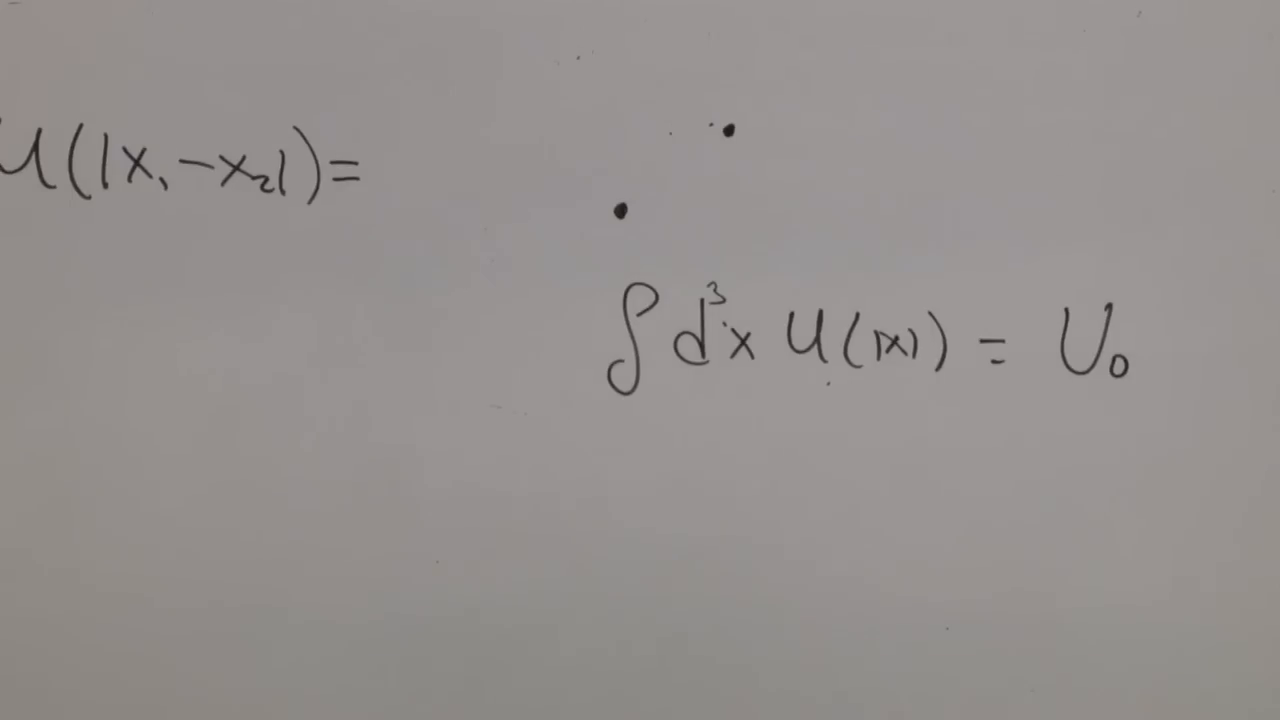
\includegraphics[width=0.90\textwidth]{lecture_06_figure_04.png}
\caption{短距離対ポテンシャルを積分された強さ\(U_0=\int d^3r\,u(r)\)に圧縮したもの。}
\lectureframe{00:25:15}
\end{figure}

\(U_0\)がなぜ有用かを知るために、一つの対を考える：
\begin{equation}
 I_2=\int_V d^3x_1\,d^3x_2\,
 u\!\left(|x_1-x_2|\right).
 \label{eq:sm6-two-particle-integral}
\end{equation}
相対座標\(r=x_2-x_1\)を導入する。境界から離れて、相対積分は\(U_0\)を与え、一方で対の共通位置は容器全体を動く。したがって
\begin{equation}
 I_2=V U_0+\text{surface corrections}.
 \label{eq:sm6-pair-integral-vu0}
\end{equation}
補正は、壁から一相互作用距離以内にある粒子から生じ、そこでは相対座標の近傍の一部が箱の外にある。その相対的な重要度は表面対体積の比としてスケールし、巨視的極限で消える。

\begin{classroomqa}
\audiencequestion{\(U_0\)は一つの選ばれた対を指すのか、そして一方の粒子は他方から固定された間隔に保たれるのか。}
\lecturerresponse{それは任意の一対に対する共通の相互作用則を指す。第一の粒子を固定し、第二の粒子をあらゆる相対位置について積分する。この積分の間、間隔は固定されていない。近傍の相互作用領域だけが有意に寄与し、\(U_0\)を生じる。
\lecturetimestamp{00:26:03--00:27:33}}
\end{classroomqa}

\begin{classroomqa}
\audiencequestion{なぜ第二の位置積分は容器全体の体積を与えるのに、第一のそれは与えないのか。}
\lecturerresponse{相対配置が\(U_0\)に積分された後、対全体は試料中を並進しうる。その共通の並進が大きな因子\(V\)を与える。相互作用近傍はすでに\(U_0\)の内部に含まれる分子スケールの体積であり、容器体積に等しい別の因子ではない。
\lecturetimestamp{00:27:48--00:29:21}}
\end{classroomqa}

\begin{classroomqa}
\audiencequestion{値はどの点を固定するかに依存しうるか、特に壁の近くではどうか。}
\lecturerresponse{並進不変性により、バルクの値は固定点に依存しない。壁の近くでは、隣接するいくつかの位置が利用できないため、積分はわずかに異なる。影響を受けるのは分子程度の厚さの表面層だけなので、箱が巨視的であれば誤差は無視できる。
\lecturetimestamp{00:29:24--00:31:22}}
\end{classroomqa}

\begin{classroomqa}
\audiencequestion{結果はすべての二粒子配置にわたって積分したポテンシャルエネルギーであり、なぜ一つの大きな体積にのみ比例するのか。}
\lecturerresponse{はい。その単位はエネルギー×体積の二乗である。なぜなら\(V U_0\)は一つの容器体積と一つの分子相互作用体積を含むからである。そのうち試料の大きさとともに増大するのは前者だけである。
\lecturetimestamp{00:31:31--00:32:04}}
\end{classroomqa}

\begin{classroomqa}
\audiencequestion{一定体積で面積を最小にする球を選ぶことは、バルクの答えを変えるか。}
\lecturerresponse{変わるのは小さな境界補正だけである。通常の巨視的な形状では、表面から分子距離以内にある粒子の数は、バルク内の粒子の数に比べて無視できる。表面が重要になるのは、容器自体が分子スケールに近づく場合だけである。
\lecturetimestamp{00:32:04--00:33:58}}
\end{classroomqa}

\begin{classroomqa}
\audiencequestion{粒子の軌道をポテンシャルに置き換えることで、衝突は省略されたのか。}
\lecturerresponse{いいえ。力はポテンシャルの導関数であり、まさに衝突を生み出すものである。平衡統計力学では、それらの衝突を一つ一つ追う必要はない。その効果はエネルギーに、したがってボルツマン重みに符号化されている。
\lecturetimestamp{00:33:59--00:35:29}}
\end{classroomqa}

\begin{classroomqa}
\audiencequestion{対力を保持しつつ真の三体相互作用を保持しないことで、何が失われるか。}
\lecturerresponse{微視的エネルギーは真の三体項を含みうるし、対ポテンシャルの高次項も多粒子相関を生み出す。しかし希薄気体中では、指定された三つの粒子が一つの分子近傍を占める確率は、二つの場合よりはるかに低い。したがって対効果が第一の密度補正を与え、より高次のクラスターは密度のより高い冪で寄与する。
\lecturetimestamp{00:35:29--00:38:14}}
\end{classroomqa}

\section{自動操縦での分配関数}

統計的手法の利点がここで見えてくる。ハミルトニアンが指定されれば、壁の近くや衝突中における詳細な速度分布を推測する必要はない。正準分配関数を書き下し、その代数をたどればよい。
\begin{equation}
\begin{aligned}
 Z&=
 \frac{1}{N!h^{3N}}
 \int d^{3N}P\,d^{3N}X\\
 &\qquad{}\times e^{-\beta K(P)}e^{-\beta U(X)},\\
 K(P)&=\sum_i\frac{p_i^2}{2m}.
\end{aligned}
 \label{eq:sm6-full-partition-function}
\end{equation}
因子\(h^{3N}\)は古典的位相空間の測度を無次元にし、\(N!\)は同種粒子の置換による過剰計数を取り除く。

\begin{figure}[t]
\centering
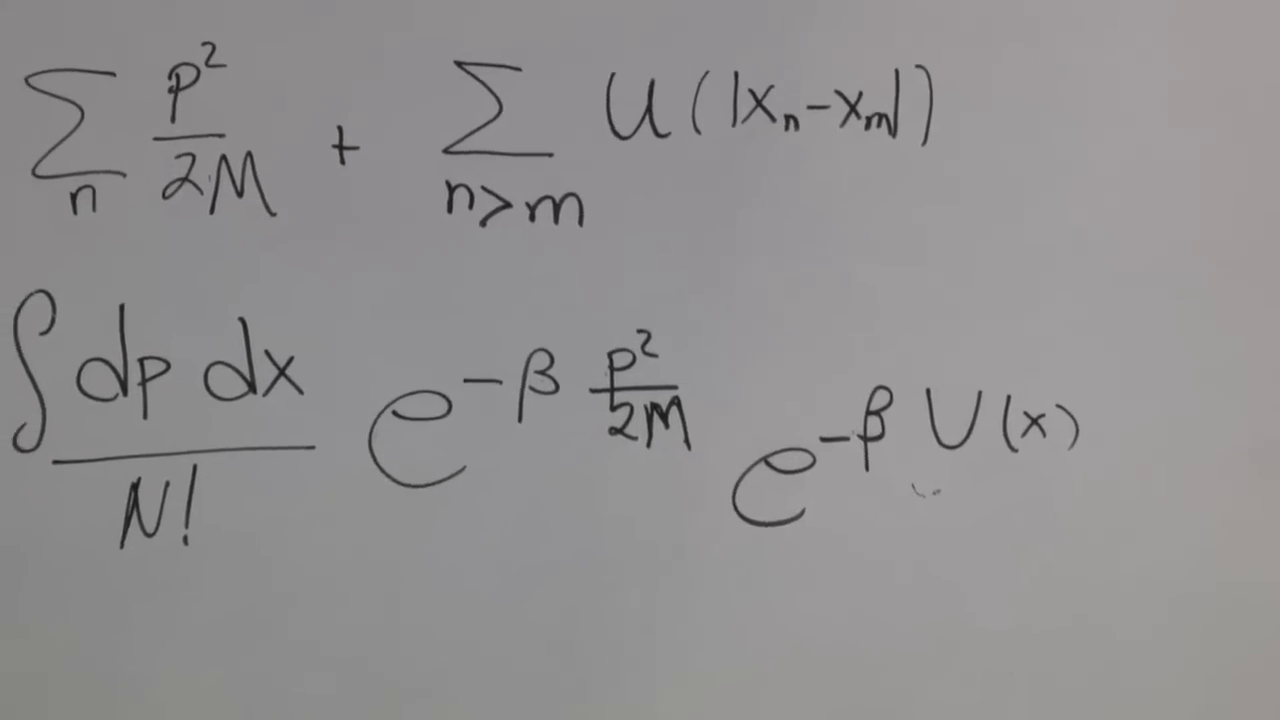
\includegraphics[width=0.90\textwidth]{lecture_06_figure_05.png}
\caption{多粒子エネルギーと、分配関数における対応する運動および配置の因子。}
\lectureframe{00:40:35}
\end{figure}

運動量と位置が分離する。配置積分に\(V^N\)を掛けて割ることで、理想気体の結果が分離される。
\begin{align}
 Z
 &=\left[
 \frac{V^N}{N!h^{3N}}
 \int d^{3N}P\,e^{-\beta K(P)}
 \right] \notag\\
 &\quad\times\left[
 \frac{1}{V^N}
 \int d^{3N}X\,e^{-\beta U(X)}
 \right] \notag\\
 &\equiv Z_0\,C(\beta,V,N).
 \label{eq:sm6-z-factorization}
\end{align}
おなじみのガウス因子は
\begin{equation}
 \int d^{3N}P\,e^{-\beta K(P)}
 =\left(\frac{2\pi m}{\beta}\right)^{3N/2}.
 \label{eq:sm6-gaussian-factor}
\end{equation}

\begin{figure}[t]
\centering
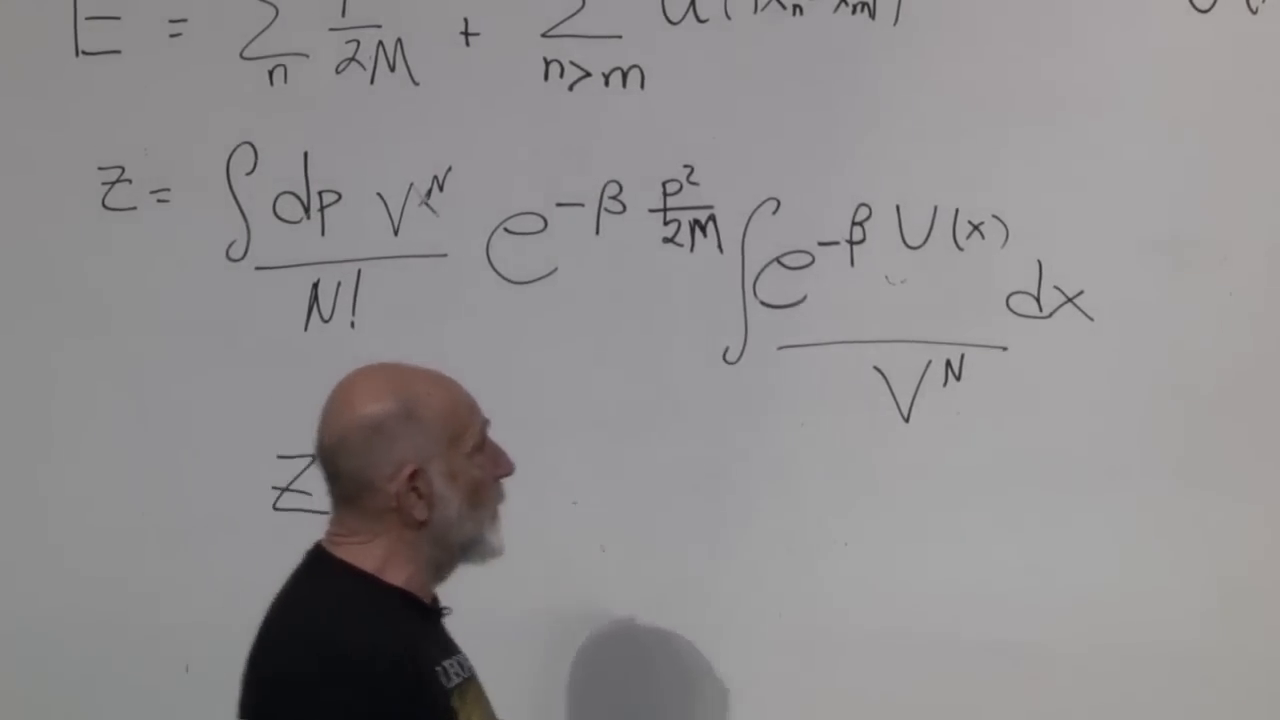
\includegraphics[width=0.90\textwidth]{lecture_06_figure_06.png}
\caption{規格化された配置因子から分離された理想気体の分配関数。}
\lectureframe{00:43:45}
\end{figure}

\(N!\)因子は規格化された比\(C\)にも、以下で用いる特定の固定\(N\)微分にも影響しないが、熱力学全体からは不要ではない。正しい状態の数え上げと示量的エントロピーにとって不可欠である。

相互作用の一次までで、
\begin{equation}
 e^{-\beta U(X)}
 =1-\beta U(X)+O(U^2).
 \label{eq:sm6-boltzmann-expansion}
\end{equation}
したがって、
\begin{align}
 C
 &=
 1-\frac{\beta}{V^N}
 \sum_{i<j}
 \int d^{3N}X\,u(|x_i-x_j|)
 +O(U^2) \notag\\
 &=
 1-\frac{\beta}{V^N}
 \frac{N(N-1)}{2}
 V^{N-2}(V U_0)+O(U^2) \notag\\
 &=
 1-\beta\frac{N(N-1)}{2V}U_0+O(U^2).
 \label{eq:sm6-configurational-correction}
\end{align}
各対は同じ\emph{積分}をもつのであり、同じ瞬間的な分離やポテンシャルエネルギーをもつのではない。残りの\(N-2\)個の位置積分はそれぞれ\(V\)の因子を一つ寄与する。

\begin{figure}[t]
\centering
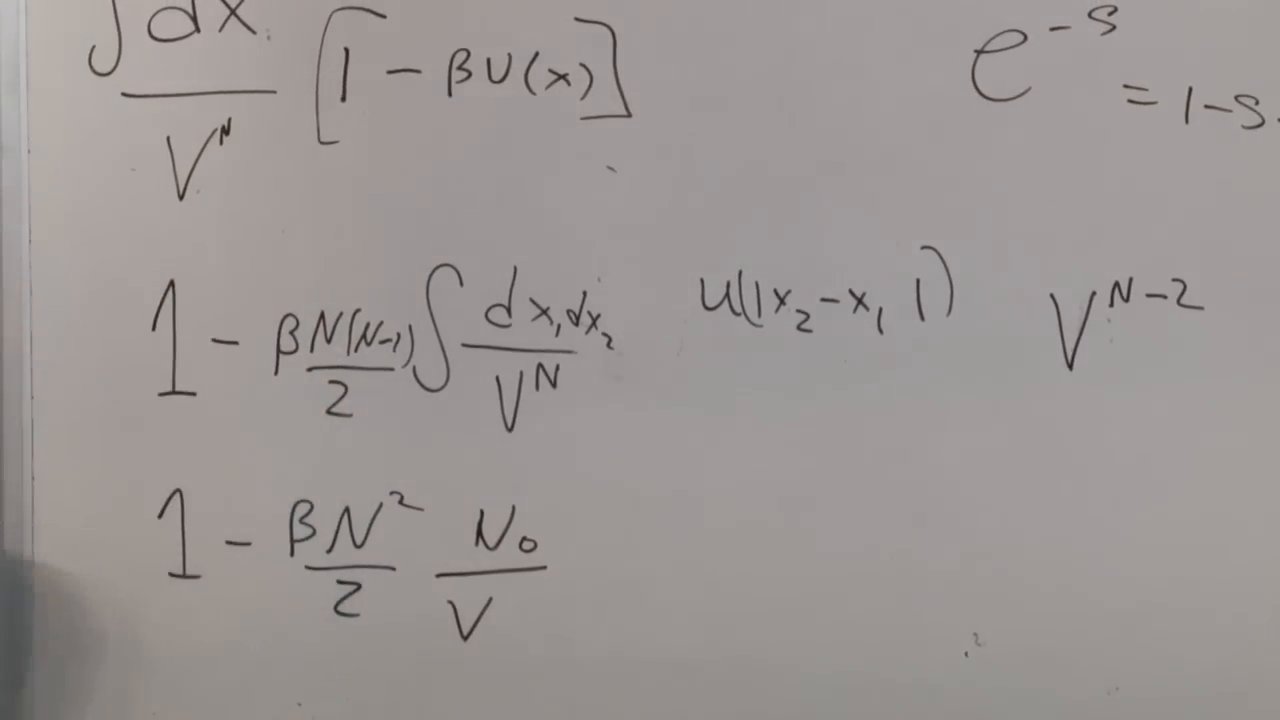
\includegraphics[width=0.90\textwidth]{lecture_06_figure_07.png}
\caption{対の数え上げ、傍観座標の体積、および第一の配置補正\(1-\beta N^2U_0/(2V)\)。}
\lectureframe{00:53:40}
\end{figure}

\begin{classroomqa}
\audiencequestion{主要な\(1\)は、分離ゼロでポテンシャルが消えることを仮定しているのか。}
\lecturerresponse{いいえ。それは指数級数のゼロ次項であり、\(u(0)\)の値に依存しない。ポテンシャルは次の項\(-\beta U(X)\)に入る。
\lecturetimestamp{00:46:19--00:46:48}}
\end{classroomqa}

\begin{classroomqa}
\audiencequestion{異なる対が異なる分離をもつのに、なぜすべての対を同じ式で置き換えてよいのか。}
\lecturerresponse{それらの点ごとの値が等しいとされているのではない。各項は同じ完全な配置空間にわたって積分され、粒子ラベルは一つの対を別の対から区別しない。積分は同一の形と同一の値をもつ。
\lecturetimestamp{00:50:00--00:51:07}}
\end{classroomqa}

\begin{classroomqa}
\audiencequestion{対の数は\(N(N-1)/2\)か、それとも
\(N(N+1)/2\)か。}
\lecturerresponse{\(N(N-1)/2\)である。一つの粒子を選んだ後には
\(N-1\)個の異なる相手しかなく、2で割ることで逆順の
順序が除かれる。巨視的な\(N\)では、\(N(N-1)\)を\(N^2\)に置き換えても
相対的な\(1/N\)の補正しか変わらない。
\lecturetimestamp{00:48:33--00:49:56}}
\end{classroomqa}

\(\log(1-x)=-x-x^2/2-x^3/3-\cdots\)は交代級数ではないので、
一次の対数は
\begin{equation}
 \log Z
 =
 \log Z_0
 -\beta\frac{N(N-1)}{2V}U_0
 +O(U^2).
 \label{eq:sm6-logz-correction}
\end{equation}
である。大きな\(N\)では、\(N(N-1)\)を\(N^2\)に置き換えてよく、そこでは有限の\(N\)による区別は必要ない。

\begin{remark}
制御された低密度の定式化では、Mayer関数
\(f(r)=e^{-\beta u(r)}-1\)と第二ビリアル係数
\begin{equation}
 B_2(T)=-\frac{1}{2}\int d^3r\,f(r).
 \label{eq:sm6-second-virial}
\end{equation}
を用いる。弱いポテンシャルに対しては\(f(r)\simeq-\beta u(r)\)なので、
\(B_2\simeq\beta U_0/2\)となり、以下の結果が回復される。この形は、\(e^{-\beta u}\)を直接展開することが
妥当でない硬い反発芯に対して必要である。
\end{remark}

\section{エネルギー、圧力、そして補正の意味}

\(Z\)の対数は、その導関数が測定可能であるため有用である。
微視的ポテンシャルが温度に依存しないと仮定すると、
\begin{align}
 E
 &=-\left(\frac{\partial\log Z}{\partial\beta}\right)_{V,N} \notag\\
 &=
 \frac{3}{2}NT
 +\frac{N(N-1)}{2V}U_0+O(U^2) \notag\\
 &\simeq
 N\left(\frac{3}{2}T+\frac{1}{2}\rho U_0\right),
 \qquad
 \rho=\frac{N}{V}.
 \label{eq:sm6-energy-correction}
\end{align}
一見非示量的な\(N^2\)には\(1/V\)が伴う。固定された
密度では\(N^2/V=N\rho\)なので、全エネルギーは系の
大きさに比例したままである。粒子あたりの余分なエネルギーが密度に比例するのは、選んだ分子が対エネルギーを獲得するのは別の
分子が近くにあるときだけだからである。

\begin{figure}[t]
\centering
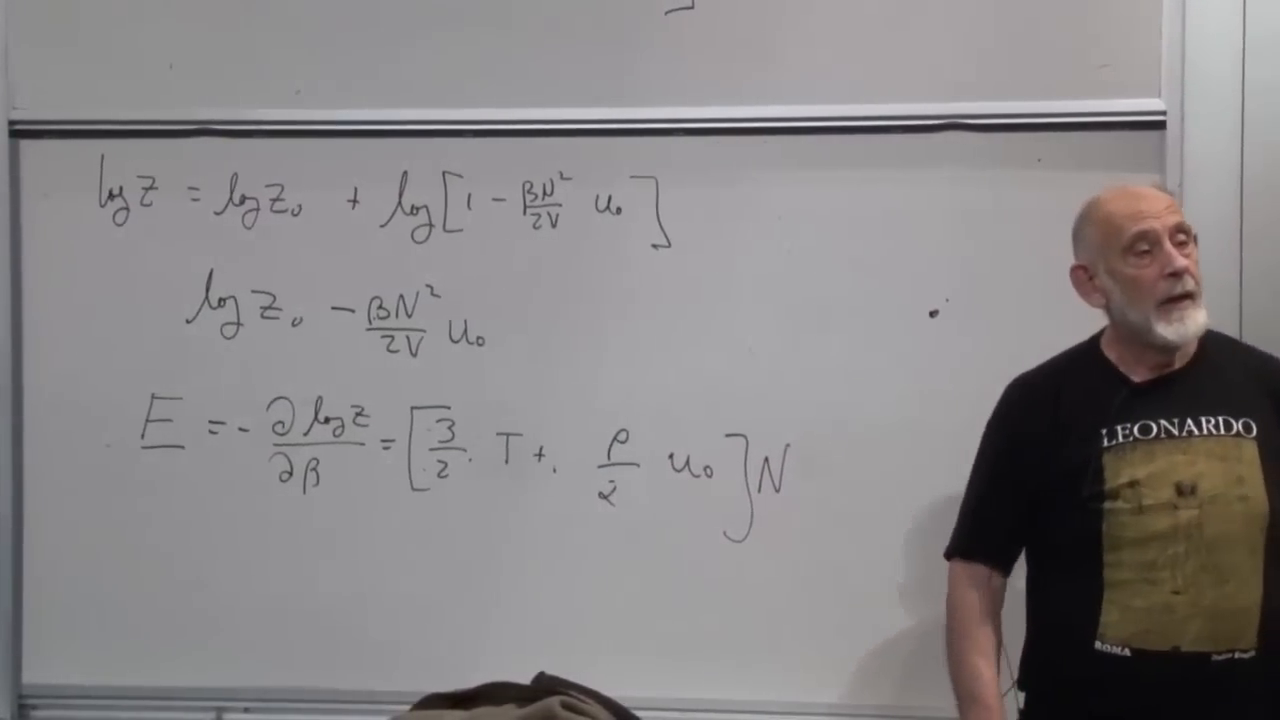
\includegraphics[width=0.90\textwidth]{lecture_06_figure_08.png}
\caption{最初の相互作用補正を示量的な
エネルギー\(N[3T/2+\rho U_0/2]\)として再編成したもの。}
\lectureframe{01:03:25}
\end{figure}

圧力の方が測定しやすい。前章の結果を用いると、
\begin{equation}
 P=T\left(\frac{\partial\log Z}{\partial V}\right)_{T,N},
 \label{eq:sm6-pressure-from-z}
\end{equation}
次を得る。
\begin{align}
 P
 &=
 \frac{NT}{V}
 +T\frac{\partial}{\partial V}
 \left(-\beta\frac{N(N-1)}{2V}U_0\right)
 +O(U^2) \notag\\
 &=
 \rho T+\frac{1}{2}\rho^2U_0
 +O\!\left(\frac{\rho U_0}{N},U^2\right).
 \label{eq:sm6-pressure-correction}
\end{align}

\begin{figure}[t]
\centering
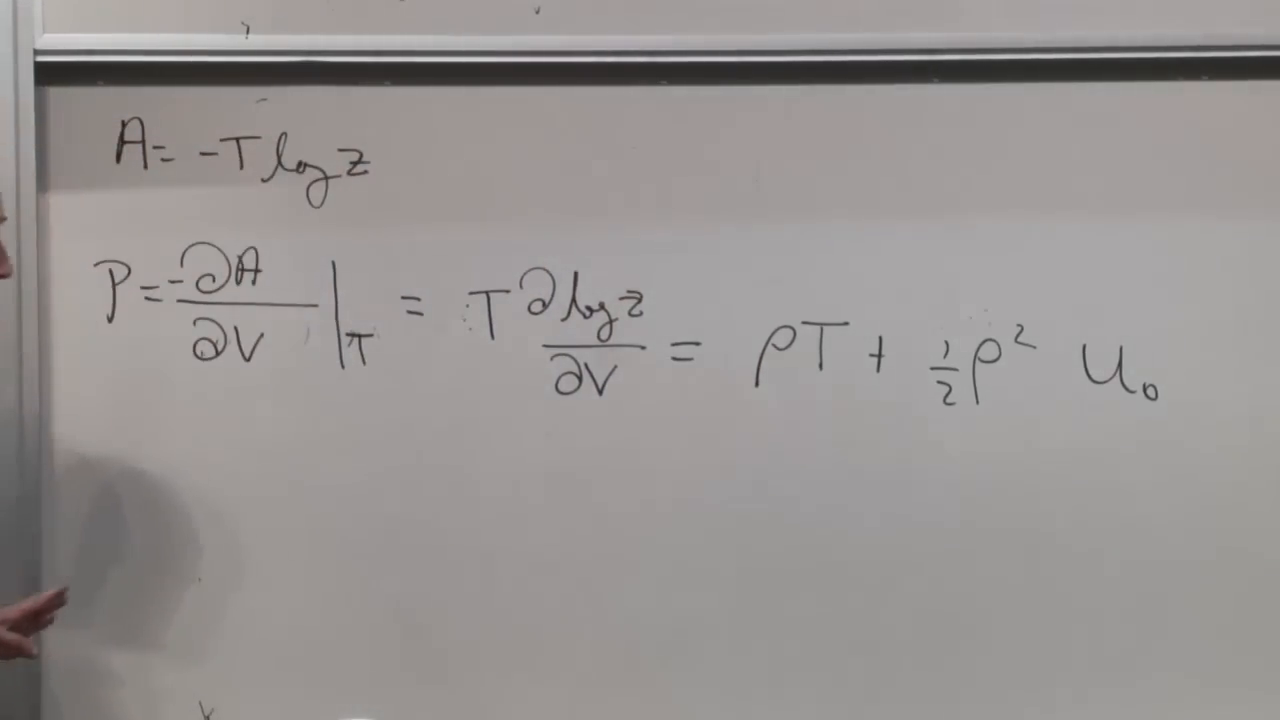
\includegraphics[width=0.90\textwidth]{lecture_06_figure_09.png}
\caption{Helmholtzの導関数から得られる圧力。最初の
密度の二次補正を含む。}
\lectureframe{01:09:50}
\end{figure}

\begin{classroomqa}
\audiencequestion{なぜ\(\rho^2\)が、別の冪ではなく、自然な
最初の補正なのか。}
\lecturerresponse{理想項は一つの粒子が
小さな領域に存在することを要し、したがって\(\rho\)のようにスケールする。相互作用は二つの
粒子が一つの分子的近傍を占めることを要し、その確率は
\(\rho^2\)のようにスケールする。因子\(1/2\)は、\((i,j)\)と\((j,i)\)が別々に数えられるのを防ぐのと同じ対の数え上げ因子である。
\lecturetimestamp{01:24:27--01:26:00}}
\end{classroomqa}

固定された温度で\(V\)を変化させ、\(\rho=N/V\)を測定し、
圧力をプロットすることができる。理想法則は線形項である。\(P(\rho)\)の曲率が
最初の相互作用補正を明らかにする。この弱ポテンシャル
近似の範囲内では、補正は明示的な温度依存性をもたない。なぜなら\eqref{eq:sm6-pressure-from-z}における因子\(T\)が
\(\beta=1/T\)を打ち消すからである。

\begin{classroomqa}
\audiencequestion{三体効果を含めなければならなくなるまで、密度はどれだけ大きくなりうるか。}
\lecturerresponse{密度の数え上げによれば、次のビリアル項は
\(\rho^3\)に比例するが、その係数は\(U_0\)だけから
推論することはできない。それは対相互作用の相関した積から、また存在するなら真の三体力から寄与を受ける。次のクラスター係数を計算し、それを\(\rho^2\)の項と比較しなければならない。推測された式を結果に昇格させるべきではない。
\lecturetimestamp{01:10:50--01:13:38}}
\end{classroomqa}

補正の大きさが小さいとき、理想気体の項が支配する。
\begin{equation}
 \begin{aligned}
 \frac{1}{2}\rho^2|U_0|&\ll \rho T,\\
 |\rho U_0|&\ll T
 \qquad\text{(parametrically)}.
 \end{aligned}
 \label{eq:sm6-ideal-validity}
\end{equation}
第二の不等式の両辺はエネルギーである。量
\(\rho U_0\)は粒子あたりの相互作用エネルギーのスケールであり、\(T\)は
運動エネルギーのスケールである。通常の希薄な室温の気体はこの領域のずっと内側にある。大きなずれが生じるのは、分子的近傍が相互作用が熱運動と競合するほど頻繁に占められるときだけである。

\begin{classroomqa}
\audiencequestion{この部屋の空気について基準を見積もることはできるか。}
\lecturerresponse{\(U_0\)を分子間相互作用エネルギーと分子体積の積として見積もり、数密度を掛け、その結果を
\(k_BT\)と比較する。粗い分子的数値は、通常の室内空気では相互作用のスケールが
はるかに小さいことを示す。分子が互いの相互作用範囲に頻繁に押し込まれるには、かなりの圧縮が必要である。
\lecturetimestamp{01:16:24--01:18:54}}
\end{classroomqa}

\begin{classroomqa}
\audiencequestion{\(U_0\)はどちらの符号もとりうるか。}
\lecturerresponse{はい。正の積分された相互作用はこの近似では正味の反発であり、圧力を\(\rho T\)より
上げる。負のそれは正味の引力であり、圧力を下げる。この符号の検査は\eqref{eq:sm6-pressure-correction}に対する即座の物理的
チェックである。
\lecturetimestamp{01:18:56--01:20:29}}
\end{classroomqa}

\begin{figure}[t]
\centering
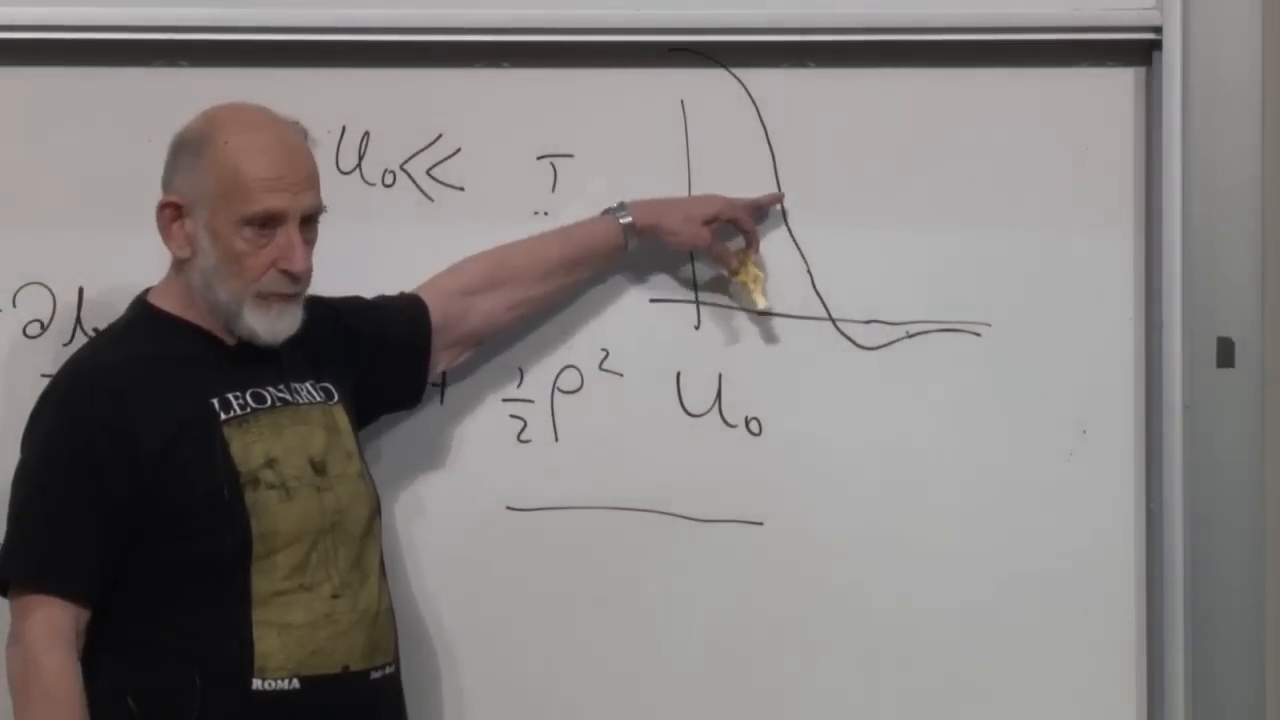
\includegraphics[width=0.90\textwidth]{lecture_06_figure_10.png}
\caption{定性的な反発および引力の対ポテンシャルプロファイルと、その補正が\(U_0\)の符号に従う圧力の式。}
\lectureframe{01:21:30}
\end{figure}

\begin{classroomqa}
\audiencequestion{静電的反発、重力引力、あるいは実際の分子間力をこの計算に組み込むことはできるか。}
\lecturerresponse{微視的ポテンシャルは原子物理学、分子物理学、あるいは量子物理学から入力される。中性分子は一般に、急峻な短距離の反発芯と、より長距離に及ぶ引力のファンデルワールス的裾を持ち、しばしば12--6ポテンシャルで模式的に表される。このような硬い芯に対しては、完全なメイヤー関数の公式を用いるべきである。重力は異なる。それは長距離的であり、その空間積分は要求される仕方では収束せず、ここで用いている通常の短距離熱力学的極限は破綻する。
\lecturetimestamp{01:20:40--01:23:03}}
\end{classroomqa}

この計算は有用な分業を例示している。微視的物理学が\(u(r)\)を与える。統計力学がそのエネルギーを\(Z\)に変え、\(Z\)の導関数がバルクの観測量を生み出し、物理的推論がその符号、密度スケーリング、示量性、妥当性の領域を検証する。形式的な操作が機械的であるのは、正しいエネルギーと近似が選ばれた後だけである。

\section{完全微分と経路依存性}

ここで数学的言語を変える。\emph{完全微分}という語句において、完全とは数値的に精密であることを意味しない。それは、1形式が真のスカラー関数の微分であることを意味する。

\(f(x,y)\)を風景の中の一点の上の高度とする。小さな変位はそれを次だけ変化させる。
\begin{equation}
 df=
 \frac{\partial f}{\partial x}\,dx+
 \frac{\partial f}{\partial y}\,dy
 =f_x\,dx+f_y\,dy.
 \label{eq:sm6-total-differential}
\end{equation}
代わりに、単に次が与えられたとしよう。
\begin{equation}
 \omega=F_x(x,y)\,dx+F_y(x,y)\,dy.
 \label{eq:sm6-one-form}
\end{equation}
\(\omega=df\)となるようなスカラー\(f\)は存在するか。混合偏導関数の等しさは次を要求する。
\begin{equation}
 \frac{\partial F_y}{\partial x}
 =
 \frac{\partial F_x}{\partial y}.
 \label{eq:sm6-exactness-condition}
\end{equation}
単連結領域上では、このゼロ回転条件は十分でもある。成分\((F_x,F_y)\)はそのとき\(f\)の勾配をなす。

\begin{figure}[t]
\centering
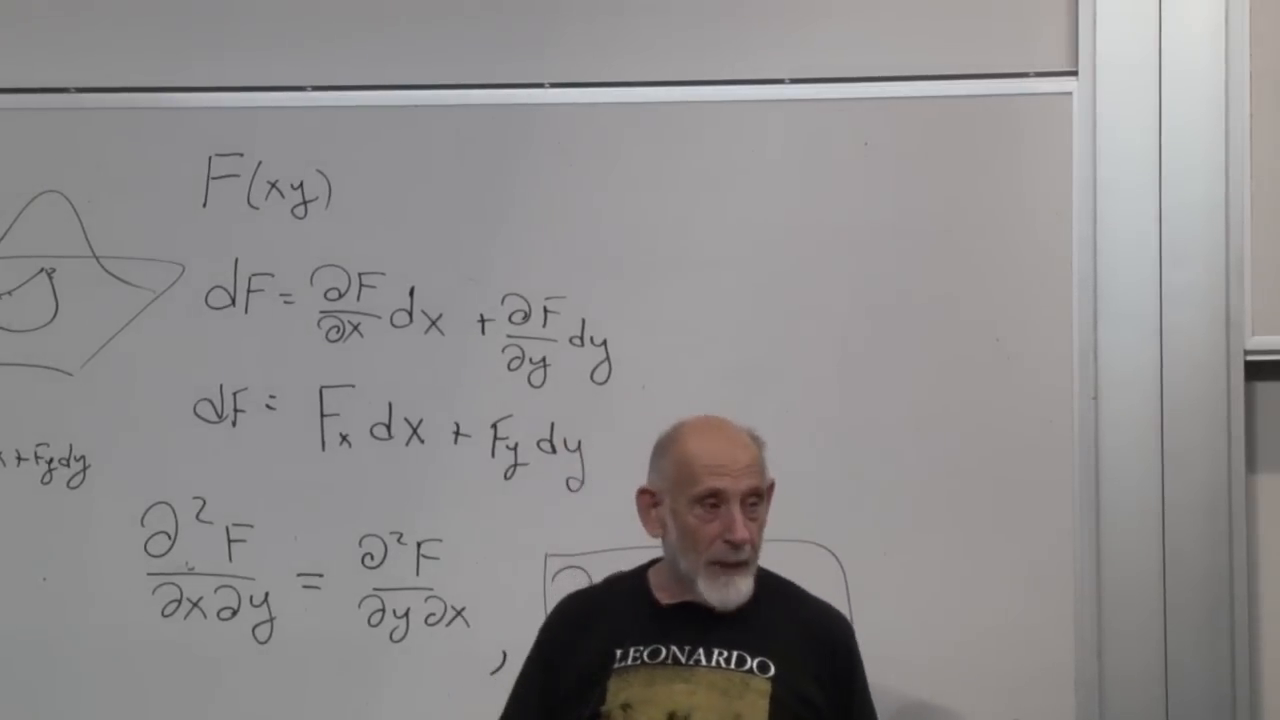
\includegraphics[width=0.90\textwidth]{lecture_06_figure_11.png}
\caption{スカラー関数としての高度、その微分、および完全性のための混合偏導関数条件。}
\lectureframe{01:34:30}
\end{figure}

同じ条件には積分的な意味がある。もし\(\omega=df\)ならば、
\begin{equation}
 \int_{\gamma:1\to2}\omega=f(2)-f(1)
 \label{eq:sm6-path-independent-integral}
\end{equation}
は端点のみに依存し、経路\(\gamma\)には依存しない。特に、
\begin{equation}
 \oint_\gamma\omega=0
 \label{eq:sm6-closed-loop-zero}
\end{equation}
がすべての可縮な閉ループに対して成り立つ。

高度はこの性質を持つ。同じ二点間を、平らな道で運転しても丘を越えて運転しても、高度の正味の変化は同じである。燃料消費はそうではない。起伏のある経路と平らな経路は一般に異なる量を消費し、閉じた旅は燃やした燃料を元に戻さない。残っている燃料の量は、拡大された状態記述においては確かに明確に定義された量であるが、それは車の位置\((x,y)\)だけの関数ではない。それは経路の記憶を伴っている。疲労も同種の類推を与える。坂を下ることは、それを登った疲労を一般には打ち消さない。

\begin{classroomqa}
\audiencequestion{完全性は保存力と同じ考えであり、曲率と関係しているのか。}
\lecturerresponse{回転がゼロの力場は局所的に保存的であり、ポテンシャルを許すので、言葉遣いは密接に関係している。平行移動と曲率もまた、閉ループの変化を局所的な幾何学的情報に結びつけるが、それはより広い主題である。ここでは初等的な主張のみが必要である。ゼロ回転は局所的な経路独立性を意味し、領域について通常の大域的條件が課される。
\lecturetimestamp{01:39:22--01:41:07}}
\end{classroomqa}

二つの例がこの判定を具体的にする。まず次を取る。
\begin{equation}
 F_x=y,\qquad F_y=x.
 \label{eq:sm6-exact-example}
\end{equation}
両方の交差導関数は\(1\)に等しく、確かに
\begin{equation}
 \omega=y\,dx+x\,dy=d(xy).
 \label{eq:sm6-exact-example-potential}
\end{equation}
次に一つの符号を変える。
\begin{equation}
 F_x=y,\qquad F_y=-x.
 \label{eq:sm6-inexact-example}
\end{equation}
すると
\begin{equation}
 \frac{\partial F_x}{\partial y}=1,
 \qquad
 \frac{\partial F_y}{\partial x}=-1,
 \label{eq:sm6-inexact-cross-derivatives}
\end{equation}
となるので、これらの二つの成分を勾配として持つスカラー\(f(x,y)\)は存在しない。

\begin{figure}[t]
\centering
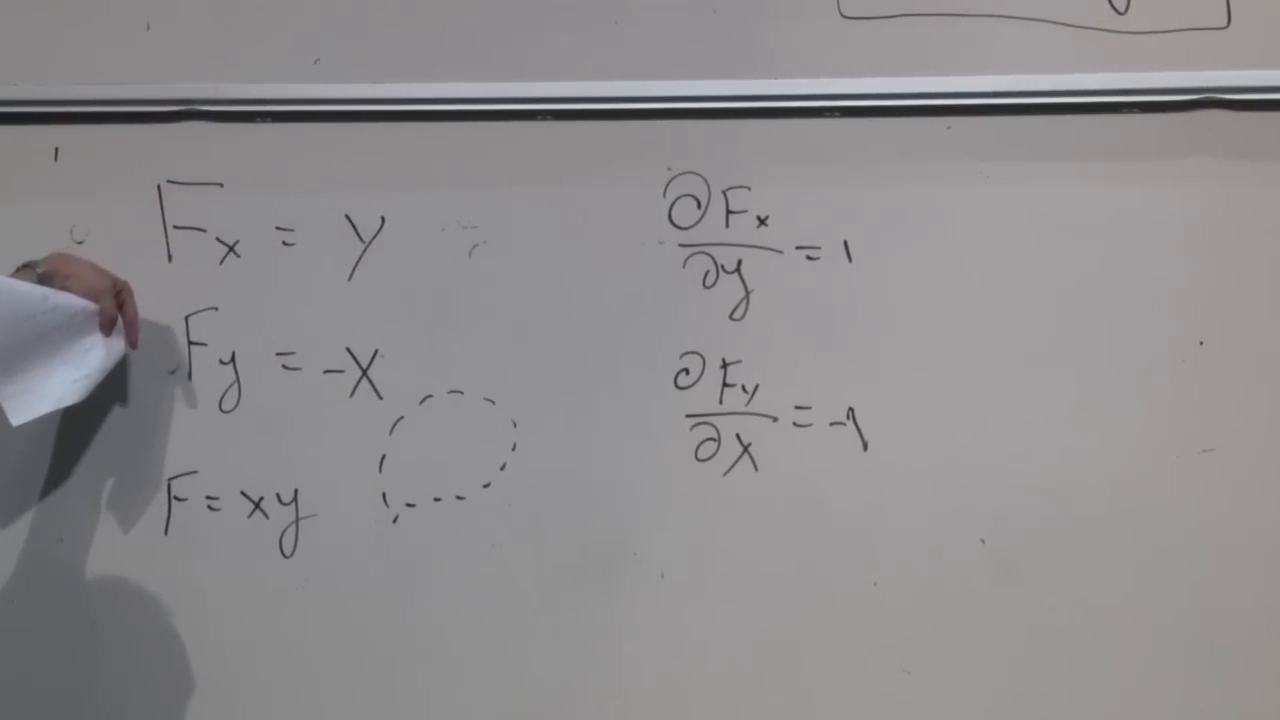
\includegraphics[width=0.90\textwidth]{lecture_06_figure_12.png}
\caption{\(f=xy\)によって生成される完全な例と、交差導関数が\(1\)および\(-1\)である不完全な例。}
\lectureframe{01:44:50}
\end{figure}

\section{熱と仕事は状態関数ではない}

粒子数が固定された単純な圧縮性系では、二つの独立な平衡変数が状態を決定する。\((T,V)\)、\((E,V)\)、あるいは、基本関係にとって特に自然な\((S,V)\)を用いてもよい。したがって
\begin{equation}
 E=E(S,V),
 \end{equation}
であり、その完全微分は
\begin{equation}
 dE=
 \left(\frac{\partial E}{\partial S}\right)_V dS+
 \left(\frac{\partial E}{\partial V}\right)_S dV
 =T\,dS-P\,dV.
 \label{eq:sm6-fundamental-relation}
\end{equation}
である。

\begin{classroomqa}
\audiencequestion{断熱とは、遅いこと、断熱されたこと、可逆であること、それともエントロピー一定であることを意味するのか。}
\lecturerresponse{この用語は文脈によって異なる使われ方をする。ここで考える平衡経路では、変化は準静的かつ熱的に断熱されており、したがって可逆かつ等エントロピーである。単に断熱された不可逆過程は依然としてエントロピーを生成しうる一方、量子断熱定理はパラメータのゆっくりした変化を強調する。
\lecturetimestamp{01:47:13--01:47:54}}
\end{classroomqa}

エントロピーを固定したとき、膨張は気体のエネルギーを
\(-P\,dV\) だけ変化させる。体積を固定したとき、可逆的な熱の移動はそれを
\(T\,dS\) だけ変化させる。したがって、次のように書くのが有用である。
\begin{equation}
 \begin{aligned}
 \delta W_{\mathrm{on}}&=-P\,dV,
 &\delta Q_{\mathrm{rev}}&=T\,dS,\\
 dE&=\delta Q_{\mathrm{rev}}+\delta W_{\mathrm{on}}.&&
 \end{aligned}
 \label{eq:sm6-first-law-increments}
\end{equation}
記号 \(\delta\) は、\(d\) ではなく、熱と仕事が状態関数の微分ではなく経路の増分であることを先取りしている。

\begin{figure}[t]
\centering
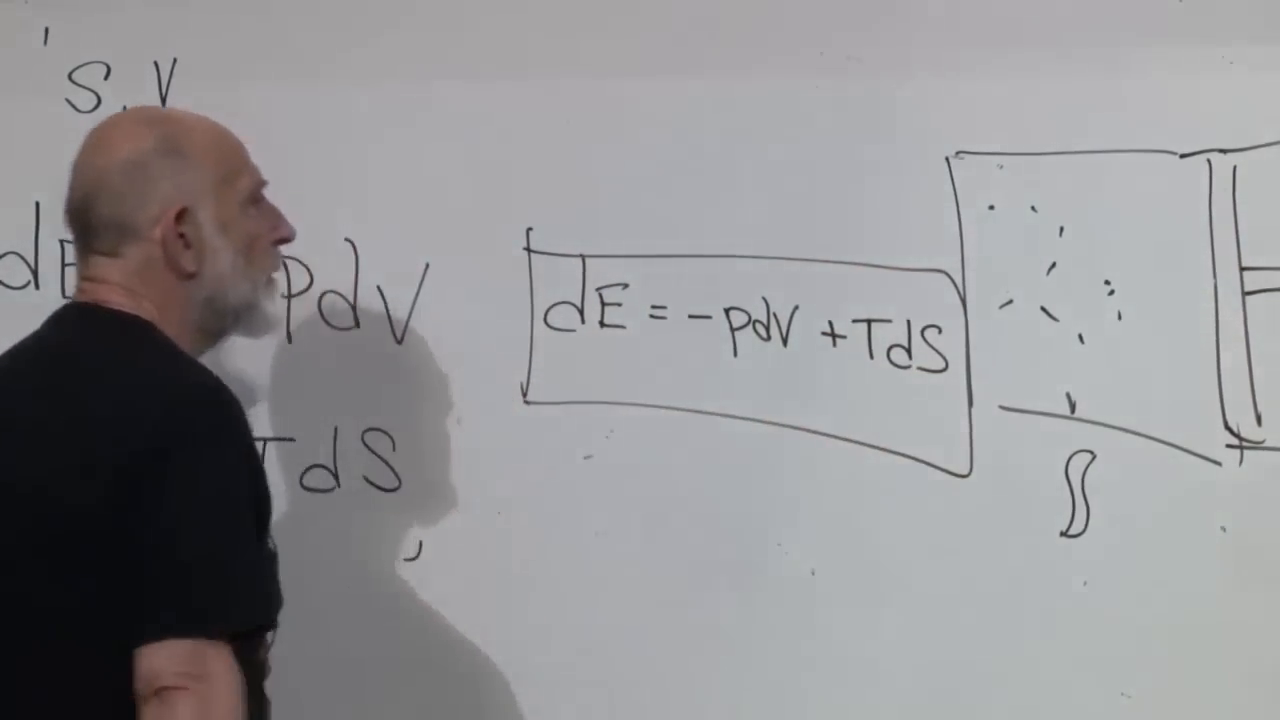
\includegraphics[width=0.90\textwidth]{lecture_06_figure_13.png}
\caption{ピストン系に対する第一法則：
\(dE=-P\,dV+T\,dS\)。}
\lectureframe{01:50:28}
\end{figure}

\begin{classroomqa}
\audiencequestion{\(-P\,dV\) は気体に対してなされる仕事を表すのか、それとも気体がなす仕事を表すのか。}
\lecturerresponse{
\eqref{eq:sm6-first-law-increments} の規約では、気体に対してなされる仕事である。膨張の間 \(dV>0\)、気体はピストンに対して正の仕事をするので、気体に対してなされる仕事は負であり、気体はエネルギーを失う。二つの記述は大きさが等しく符号が反対である。
\lecturetimestamp{01:51:23--01:52:27}}
\end{classroomqa}

等式 \(\delta Q_{\mathrm{rev}}=T\,dS\) を、そのまま任意の不可逆加熱に拡張してはならない。一般には、
\begin{equation}
 dS=\frac{\delta Q}{T_{\mathrm{boundary}}}+dS_{\mathrm{prod}},
 \qquad dS_{\mathrm{prod}}\ge 0.
 \label{eq:sm6-entropy-production}
\end{equation}
以下に述べる完全微分の議論は準静的平衡経路に関するものであり、その場合には可逆関係が適切である。

\begin{classroomqa}
\audiencequestion{状態空間の議論におけるすべての経路は、平衡状態を通ると仮定されているのか。}
\lecturerresponse{はい。操作は十分にゆっくり行われるので、\(P\)、\(T\)、\(E\)、\(S\)、\(V\) は経路に沿って well-defined のままである。熱と仕事の経路依存性は、系が平衡から遠く離れて駆動されることを必要としない。
\lecturetimestamp{01:54:30--01:54:39}}
\end{classroomqa}

熱が完全微分であるかどうかを調べるには、\((E,V)\) を座標として用い、第一法則を整理する。
\begin{equation}
 \delta Q_{\mathrm{rev}}=dE+P(E,V)\,dV.
 \label{eq:sm6-heat-one-form}
\end{equation}
もし \(dQ=\delta Q_{\mathrm{rev}}\) となる状態関数 \(Q(E,V)\) が存在するならば、その偏導関数は
\begin{equation}
 \left(\frac{\partial Q}{\partial E}\right)_V=1,
 \qquad
 \left(\frac{\partial Q}{\partial V}\right)_E=P.
 \label{eq:sm6-hypothetical-heat-derivatives}
\end{equation}
でなければならない。そのとき混合導関数の等しさは
\begin{equation}
 \begin{aligned}
 \frac{\partial}{\partial V}
 \left(\frac{\partial Q}{\partial E}\right)_V
 &=\frac{\partial}{\partial E}
 \left(\frac{\partial Q}{\partial V}\right)_E,\\
 0&=\left(\frac{\partial P}{\partial E}\right)_V.
 \end{aligned}
 \label{eq:sm6-heat-exactness-requirement}
\end{equation}
を要求する。

\begin{classroomqa}
\audiencequestion{これは \(F_x\,dx+F_y\,dy\) に用いられるのとまさに同じ回転テストか。}
\lecturerresponse{はい。\(dE\) と \(dV\) の係数は \(1\) と
\(P(E,V)\) である。それらの交差導関数は \(0\) と
\((\partial P/\partial E)_V\) である。熱が完全微分であるのは、それらの導関数が一致する場合に限られる。
\lecturetimestamp{01:54:39--01:54:52}}
\end{classroomqa}

\begin{figure}[t]
\centering
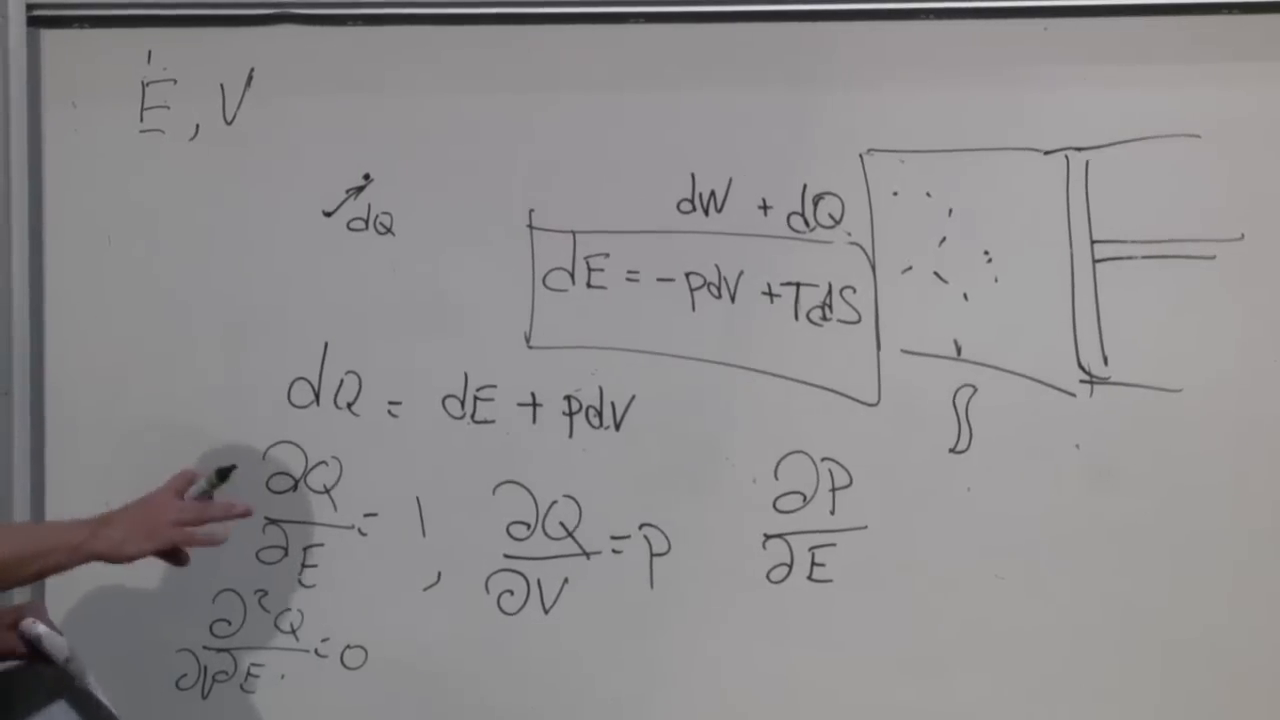
\includegraphics[width=0.90\textwidth]{lecture_06_figure_14.png}
\caption{熱の一次形式 \(dE+P\,dV\) と、それが状態関数の微分である場合に要求される混合導関数。}
\lectureframe{01:58:10}
\end{figure}

この要求はすでに物理的にありそうにない。体積を固定して気体にエネルギーを加えると、一般にはその圧力が変化する。理想気体は直接的な計算を与える。
\begin{equation}
 PV=NT,
 \qquad
 E=\frac{3}{2}NT
 \quad\Longrightarrow\quad
 P=\frac{2E}{3V}.
 \label{eq:sm6-ideal-pressure-energy}
\end{equation}
したがって
\begin{equation}
 \left(\frac{\partial P}{\partial E}\right)_V
 =\frac{2}{3V}\ne0.
 \label{eq:sm6-heat-curl-fails}
\end{equation}
回転テストは失敗する。\(\delta Q_{\mathrm{rev}}\) は完全微分ではない。仕事の増分 \(\delta W_{\mathrm{on}}=-P\,dV\) も同じ理由で失敗する。

\begin{figure}[t]
\centering
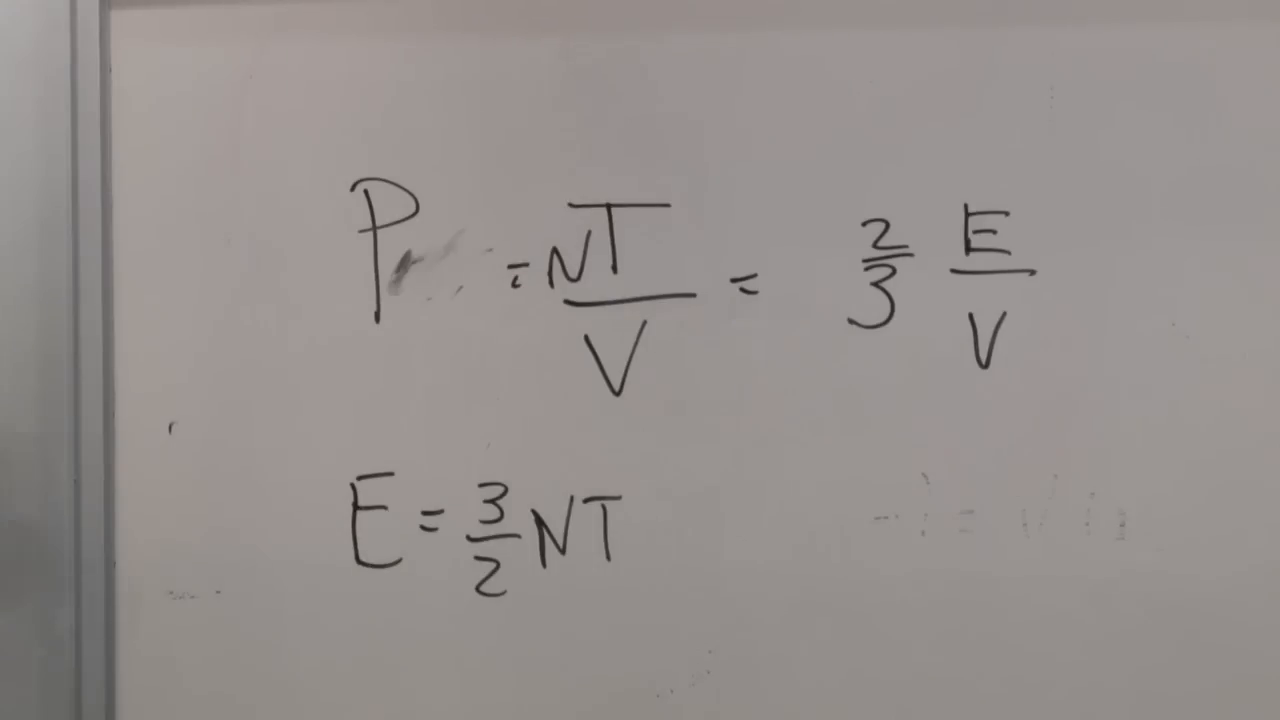
\includegraphics[width=0.90\textwidth]{lecture_06_figure_15.png}
\caption{理想気体の関係を組み合わせると
\(P=2E/(3V)\) となる。}
\lectureframe{02:00:00}
\end{figure}

\begin{figure}[H]
\centering
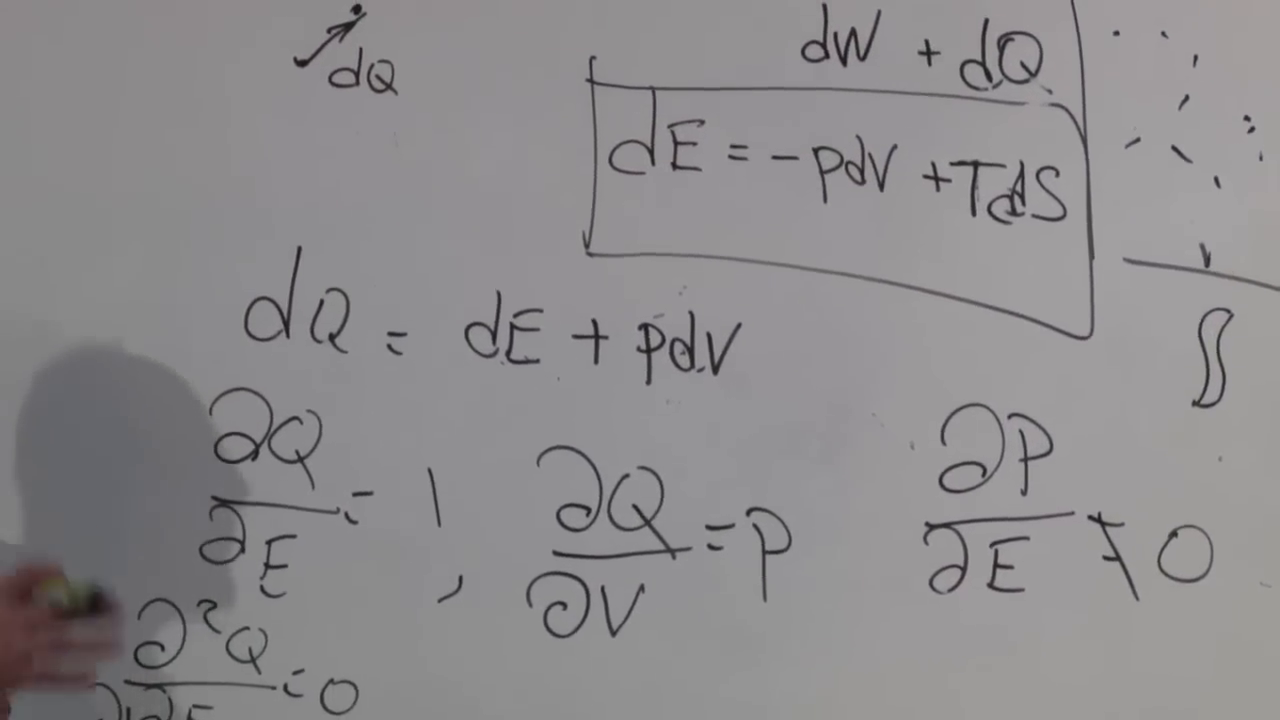
\includegraphics[width=0.90\textwidth]{lecture_06_figure_16.png}
\caption{完成した議論：\((\partial P/\partial E)_V\ne0\) であるから、熱の一次形式は完全微分でありえない。}
\lectureframe{02:00:35}
\end{figure}

閉じた平衡サイクルに対して、
\begin{equation}
 \oint dE=0,
 \qquad
 \oint\delta Q_{\mathrm{rev}}
 =-\oint\delta W_{\mathrm{on}}.
 \label{eq:sm6-cycle-balance}
\end{equation}
系は同じエネルギーに戻るが、熱と仕事は別々に消える必要はない。それらの値は状態空間を通る経路に依存する。これが、作動物質が初期の熱力学的状態に戻るにもかかわらず、サイクル機関が熱を吸収して正味の仕事を供給できる理由である。

\begin{classroomqa}
\audiencequestion{この経路依存性は、機関効率、ヒステリシス、記憶と関係しているのか。}
\lecturerresponse{機関サイクルはそれを直接利用する。閉サイクルの熱入力は、状態関数 \(E\) が初期値に戻る間、正味の仕事出力と釣り合う。ヒステリシスと記憶も経路依存性を含むが、それらはしばしば追加の内部変数や非平衡物理を必要とする。現在の結論はより狭く、すでに可逆平衡経路に対して成り立つ。熱と仕事は移動であり、熱力学的状態に蓄えられた性質ではない。
\lecturetimestamp{02:02:21--02:03:17}}
\end{classroomqa}

議論の二つの半分がここで出会う。測定は、その制御と平衡条件が指定されて初めて意味を持つ。近似は、その小さなパラメータと失敗基準が指定されて初めて意味を持つ。熱力学量は、その微分が経路非依存性のテストに合格して初めて状態関数である。いずれの場合も、規律ある数学は物理的解釈を置き換えるのではなく、その解釈がどこで正当化されるかを正確に教えてくれる。